%!TEX root = ../Fast_Contour_Tracing_Algorithm.tex
% -*- root: ../Fast_Contour_Tracing_Algorithm.tex -*-

\section{Experimental Result}

% For comparing the proposed algorithm with conventional algorithms, we perform experiment for determining their accuracy, speed, and stored data size. Table \ref{table:exp_environment} shows the experimental environment.

To compare the proposed algorithm with conventional algorithms, we perform an experiment to determine their accuracy, speed, and stored data size. Table \ref{table:exp_environment} shows the experimental environment.

\begin{table}[h]
	\centering
	\begin{tabularx}{0.9\textwidth}{L{4cm}L{20cm}}
		\toprule
		  &  Desktop \\ 
		\midrule
		CPU & Intel\textregistered~ Core\texttrademark~i7-2600K CPU @ 3.40GHz  \\
		Memory & 14.0 GB \\  
		HDD & Seagate 1TB Momentus ST1000LM024 \\
		O/S & Microsoft Windows 7 \\
		Development & Microsoft Visual Studio 2013 \\ 
		\bottomrule
	\end{tabularx}
	\caption{Experimental Environment}
	\label{table:exp_environment}
\end{table}	

% We experimented on nine CCITT standard fax images with 200 DPI (dots per inch) \cite{Miyatake1997Contour}. All these images have $1,728 \times 2,339$ pixels and a file size of 11,842 KB. Table \ref{table:ccitt} shows the document type of these images and the total number of contour pixels. We used these large sized images because they a number of various types of contours, and they are useful to compare the efficiencies with regard to parameters such as processing time and accuracy of the trace results of the contour tracing algorithms.

We experimented on nine CCITT standard fax images with 200 dots per inch (dpi) \cite{Miyatake1997Contour}. All of these images have $1,728 \times 2,339$ pixels and a file size of $11,842 KB$. Table \ref{table:ccitt} shows the document type of these images and the total number of contour pixels. We used these large-sized images because they have various types of contours, which is useful when comparing the efficiencies with regard to parameters such as processing time and the accuracy of the trace results of the contour-tracing algorithms.

\begin{table}[h]
	\centering
	\begin{tabularx}{1.0\textwidth}{C{3cm}YY}
		\toprule
		Index & Type & Total number of contour pixels \\
		\midrule
		1 & Business letter & 81,189 \\
		2 & Circuit diagram & 50,825 \\
		3 & Sales order table & 152,489 \\
		4 & French document & 312,812 \\
		5 & Technical paper & 157,377 \\
		6 & Technical graph & 98,579 \\
		7 & Japanese document & 283,717 \\
		8 & Handwritten memo & 97,031 \\
		9 & Facsimile test chart & 453,721 \\
		\bottomrule
	\end{tabularx}
	\caption{CCITT Fax Standard Images}
	\label{table:ccitt}
\end{table}	

% In order to compare the proposed algorithm with conventional algorithms, we used the experimental method described in \cite{Danielsson1981Improvement} for determining the start pixels of the outer and inner contours of the images. In other words, whenever any untraced contour pixel is searched using a raster scan from the left-top to the right-bottom of the images, this pixel is regarded as the start pixel and the tracer starts contour tracing. If the contour is an outer contour, the tracer's initial direction is assigned as East (``E''). On the contrary, in the case of the inner contour of an object e.g., ``e,'' ``p,'' ``q,'' ``R,'' and ``o,'' the tracer's initial direction is assigned as West (``W''), as shown in figure \textcolor{red}{2 (a)}.

In order to compare the proposed algorithm with conventional algorithms, we used the experimental method described in Ref. \cite{Danielsson1981Improvement} to determine the start pixels of the outer and inner contours of the images. In other words, whenever any untraced contour pixel is searched using a raster scan from the left top to the right bottom of the images, this pixel is regarded as the start pixel, and the tracer starts contour tracing. If the contour is an outer contour, the tracer's initial direction is assigned as East (``E''). On the contrary, in the case of the inner contour of an object, e.g., ``e,'' ``p,'' ``q,'' ``R,'' and ``o,'' the tracer's initial direction is assigned as West (``W''). 

% In the experiments, we did not consider the TPA, since the initial condition of the TPA\cite{Ghuneim2015Contour,Pavlidis2012Algorithms} is that it must start with white left (``L''), left-rear (``W''), and right-rear (``R'') pixels, which is not satisfied in some of the inner contours. Figure \ref{fig:image15} shows an example of this violation. In our experimental situation, there were many cases in which such conditions were not satisfied; therefore, we could not perform identical experiments and meaningful data was not obtained for comparing the trace results with those of the other methods. 

In the experiments, we did not consider the TPA because the initial condition of the TPA \cite{Ghuneim2015Contour,Pavlidis2012Algorithms} is that it must start with white left (``L''), left-rear (``W''), and right-rear (``R'') pixels, which is not satisfied in some of the inner contours. Figure \ref{fig:image15} shows an example of this violation. In our experiments, there were many cases for which these conditions were not satisfied. Therefore, we could not perform identical experiments, and meaningful data were not obtained for comparing the trace results with those of the other methods. 

%%% Figure 15
\begin{figure}[htbp]
	\centering
	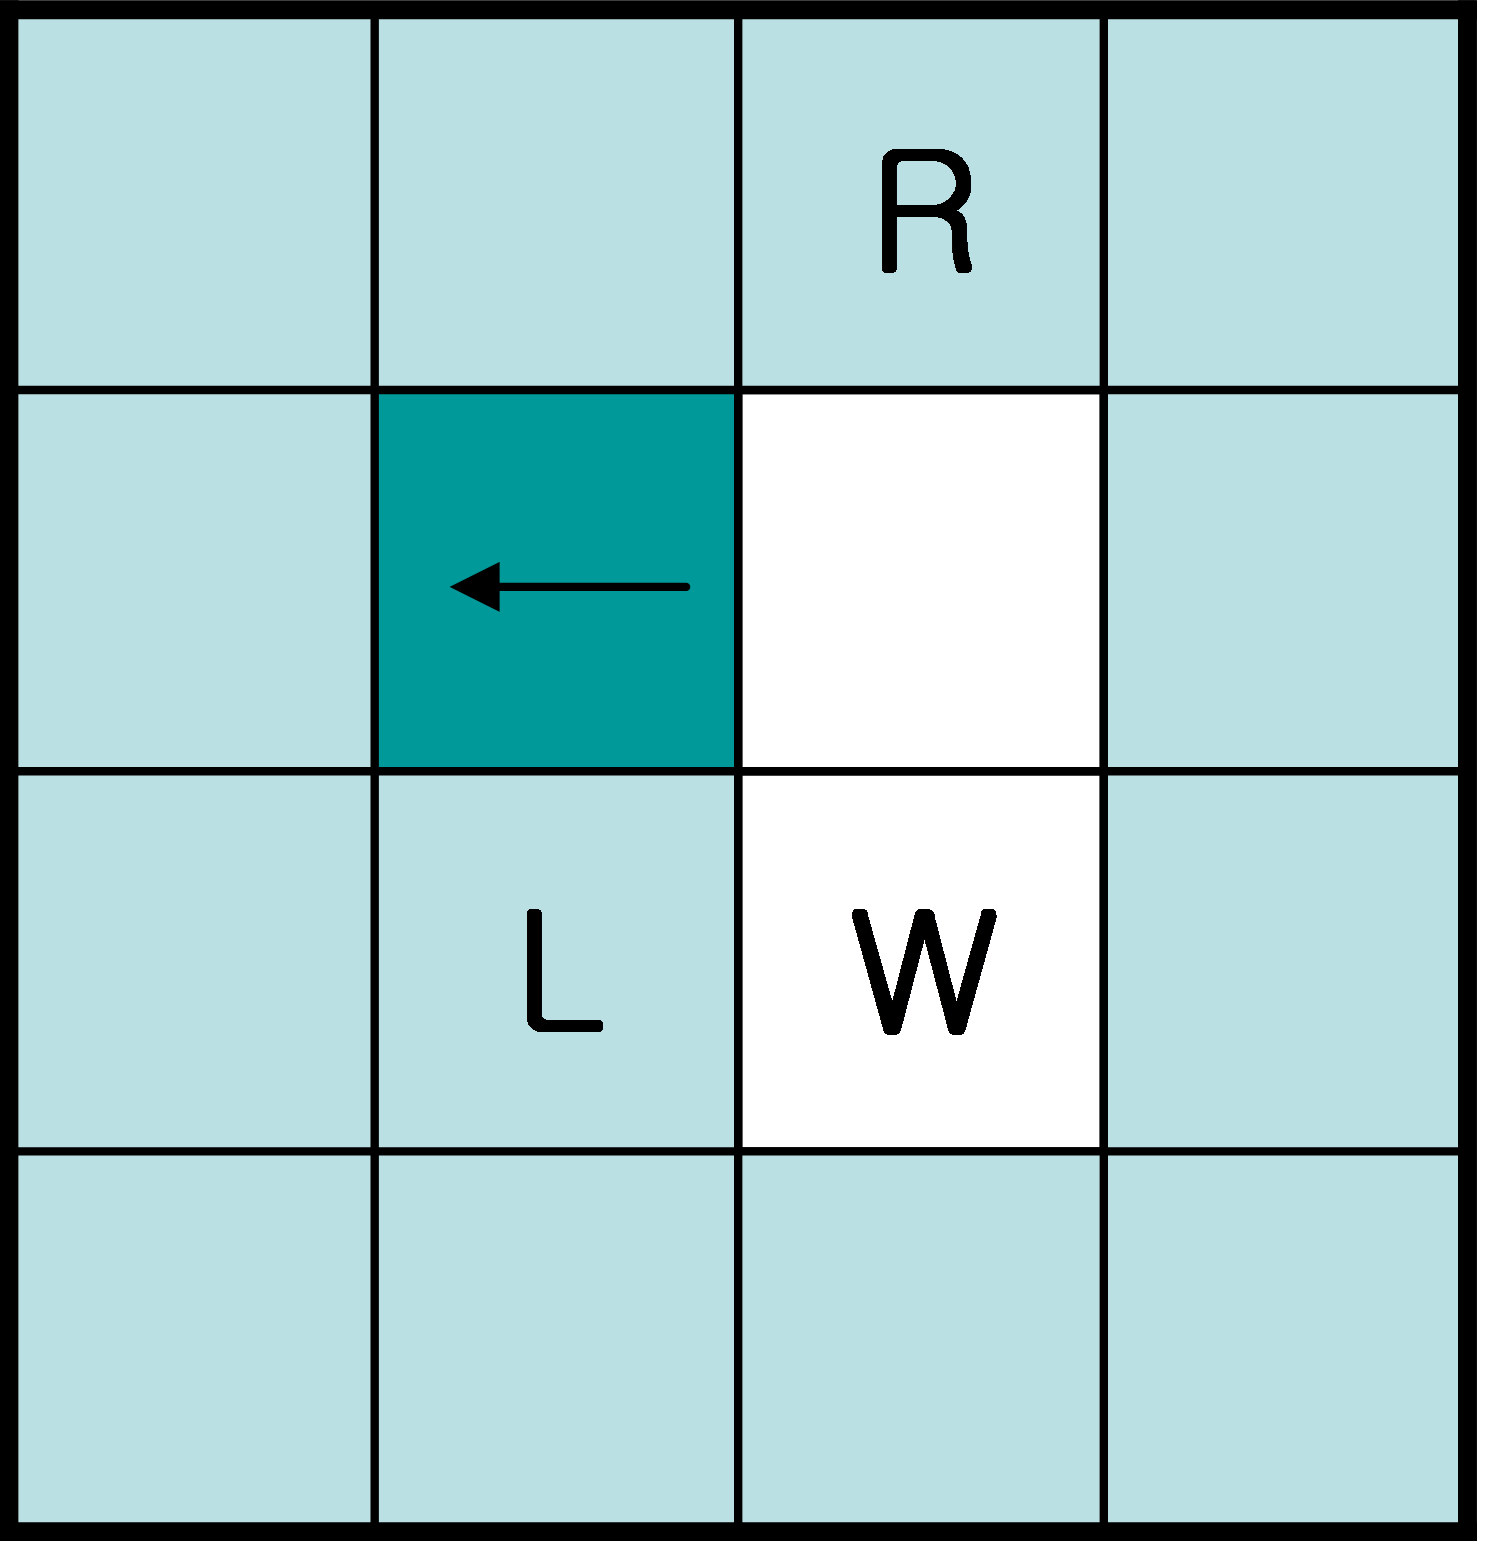
\includegraphics[width=0.3\textwidth]{5.ExperimentalResult/fig15.png}
	\caption{Problem with TPA.}
	\label{fig:image15}
\end{figure}

\subsection{Accuracy}

% The accuracy of contour tracing involves determining how accurately the tracing algorithm traces, and we measure it by counting the number of pixels traced. Firstly, we apply each algorithm to the test images and mark the tracing on the images. Then we count all the marked contour pixels in the images. Therefore, even if a pixel is traced several times, it is counted only once. Table \JHMEMO{7} shows the results of the comparison between the proposed algorithm and the conventional ones. In the table, \JHMEMO{``total number''} implies the total number of contour pixels, including the inner corner, outer corner, inner-outer corner, and straight line pixels. In this result, the MNT and RSA traced the least number of pixels as contours because they could not trace the inner corner pixels. the SBF has inconsistencies with regard to the inner-outer corner and inner corner types; therefore, it traced lesser number of pixels as compared to the ISBF and proposed algorithm.  Further, the MSBF has inner corner inconsistencies that are similar to those of the SBF; the MSBF traced lesser number of pixels as compared to the proposed algorithm and ISBF. The proposed algorithm shows that $99.5\%$ of the total contour pixels were found to be the same as those in the case of the ISBF and it has the maximum total number of traced contour pixels. In conclusion, the proposed algorithm produced the best results with regard to tracing accuracy.

%%% Table 7
%!TEX root = ../Fast_Contour_Tracing_Algorithm.tex
% -*- root: ../Fast_Contour_Tracing_Algorithm.tex -*-

% Please add the following required packages to your document preamble:
% \usepackage{multirow}
\begin{table}[]
\centering
\caption{Comparison of Traced Contour Pixels.}
\label{table:table7}
\resizebox{\textwidth}{!}{%

\begin{tabular}{llllllllllllll}

\toprule

\multirow{2}{*}{Image} & \multirow{2}{*}{Total Number} & \multicolumn{2}{l}{Proposed} & \multicolumn{2}{l}{ISBF} & \multicolumn{2}{l}{MSBF} & \multicolumn{2}{l}{SBF} & \multicolumn{2}{l}{MNT} & \multicolumn{2}{l}{RSA} \\

                       &                               & Number          & \%         & Number        & \%       & Number        & \%       & Number        & \%      & Number        & \%      & Number        & \%      \\

\midrule

\#1                    & 81,189                        & 81,188          & 100.0      & 81,188        & 100.0    & 73,743        & 90.8     & 73,613        & 90.7    & 65,503        & 80.7    & 65,503        & 80.7    \\
\#2                    & 50,825                        & 50,824          & 100.0      & 50,824        & 100.0    & 45,003        & 88.5     & 45,003        & 88.5    & 38,819        & 76.4    & 38,819        & 76.4    \\
\#3                    & 152,489                       & 152,487         & 100.0      & 152,487       & 100.0    & 139,589       & 91.5     & 139,589       & 91.5    & 126,414       & 82.9    & 126,414       & 82.9    \\
\#4                    & 312,812                       & 312,812         & 100.0      & 312,812       & 100.0    & 283,709       & 90.7     & 283,712       & 90.7    & 253,169       & 80.9    & 253,169       & 80.9    \\
\#5                    & 157,377                       & 157,374         & 100.0      & 157,374       & 100.0    & 142,447       & 90.5     & 142,453       & 90.5    & 127,306       & 80.9    & 127,306       & 80.9    \\
\#6                    & 98,579                        & 98,566          & 100.0      & 98,566        & 100.0    & 91,176        & 92.5     & 91,174        & 92.5    & 82,239        & 83.4    & 82,239        & 83.4    \\
\#7                    & 283,717                       & 283,551         & 99.9       & 283,551       & 99.9     & 264,108       & 93.1     & 264,067       & 93.1    & 238,533       & 84.1    & 238,533       & 84.1    \\
\#8                    & 97,031                        & 97,015          & 100.0      & 97,015        & 100.0    & 86,822        & 89.5     & 86,822        & 89.5    & 76,251        & 78.6    & 76,251        & 78.6    \\
\#9                    & 453,721                       & 445,975         & 98.3       & 445,972       & 98.3     & 417,687       & 92.1     & 417,735       & 92.1    & 361,439       & 79.7    & 361,439       & 79.7    \\
\midrule
Total                  & 1,687,740                     & 1,679,792       & 99.5       & 1,679,789     & 99.5     & 1,544,284     & 91.5     & 1,544,168     & 91.5    & 1,369,673     & 81.2    & 1,369,673     & 81.2   \\

\bottomrule

\end{tabular}
}
\end{table}

The accuracy of contour tracing involves determining how accurately the tracing algorithm traces, and we measure it by counting the number of pixels traced. First, we apply each algorithm to the test images and mark the tracing on the images. Then, we count all the marked contour pixels in the images. Therefore, even if a pixel is traced several times, it is counted only once. Table \ref{table:table7} shows the results of the comparison between the proposed algorithm and the conventional ones. In the table, ``Total number'' implies the total number of contour pixels, including the inner corner, outer corner, inner-outer corner, and straight-line pixels. In this result, the MNT and RSA traced the least number of pixels as contours because they could not trace the inner-corner pixels. The SBF has inconsistencies with regard to the inner-outer corner and inner-corner types. Therefore, it traced fewer pixels when compared to the ISBF and proposed algorithm. Further, the MSBF has inner-corner inconsistencies that are similar to those of the SBF, and the MSBF traced fewer pixels when compared to the proposed algorithm and ISBF. The proposed algorithm shows that $99.5\%$ of the total contour pixels were found to be the same as those in the case of the ISBF, and it has the maximum total number of traced contour pixels. In conclusion, the proposed algorithm produced the best results with regard to tracing accuracy.

%%% Figure 16
\begin{figure}[htbp]
	\centering
	\subfloat[]{ 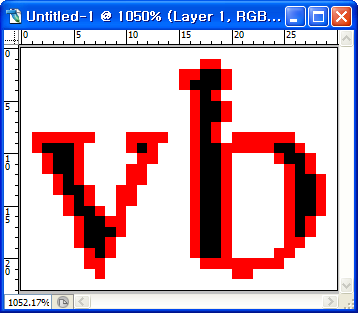
\includegraphics[width=0.3\textwidth]{5.ExperimentalResult/fig16-a.png} \label{fig:img16-a} }
	\subfloat[]{ 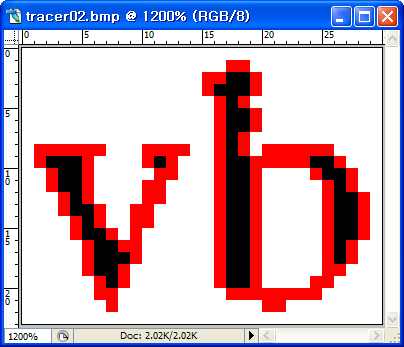
\includegraphics[width=0.3\textwidth]{5.ExperimentalResult/fig16-b.png} \label{fig:img16-b} }

	\caption{\JHMEMO{Visual comparison of two Contour Tracing Methods.} \protect\subref{fig:img16-a} MSBF \protect\subref{fig:img16-b} Proposed method}
	\label{fig:image16}
\end{figure}

% Figure 16 shows the traced images resulting from the MSBF and proposed algorithm. In this figure, (a) could not trace some of the inner corner pixels but (b) traced all the corner pixel types without any inconsistency. Moreover, as the proposed algorithm can classify each corner type, it can trace the selected type of contour pixels by omitting some cases, as shown in figure 9 (b). For example, if we remove the tracing cases (1) and (6) from the other cases, we can obtain a result without inner corner tracing, and it is the same as the result of the MNT and RSA. Figure \textcolor{red}{17 (b)} shows an image that is traced using the proposed algorithm without inner corners, and it shows that the image is consistently traced without inner corners.

Figure \ref{fig:image16} shows the traced images resulting from the MSBF and proposed algorithm. \JHMEMO{As shown in figure \ref{fig:img16-a}, MSBF was not able to trace some of the inner corner pixels, but our proposed method (figure \ref{fig:img16-b}) was able to trace all the corner-pixel types without any inconsistency.} Moreover, as the proposed algorithm can classify each corner type, it can trace the selected type of contour pixels by omitting some cases, as shown in Figure \ref{fig:img9-b}. For example, if we remove the tracing cases (1) and (6) from the other cases, we can obtain a result without inner-corner tracing, and it is the same as the result of the MNT and RSA. Figure \ref{fig:img17-b} shows an image that was traced using the proposed algorithm without inner corners, and it shows that the image is consistently traced without inner corners.

%%% Figure 17
\begin{figure}[htbp]
	\centering
	\subfloat[]{ 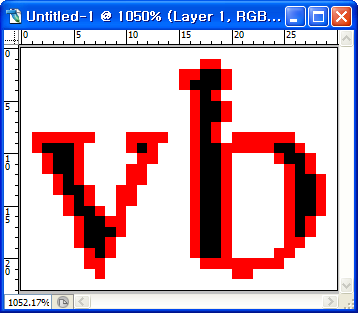
\includegraphics[width=0.3\textwidth]{5.ExperimentalResult/fig17-a.png} \label{fig:img17-a} }
	\subfloat[]{ 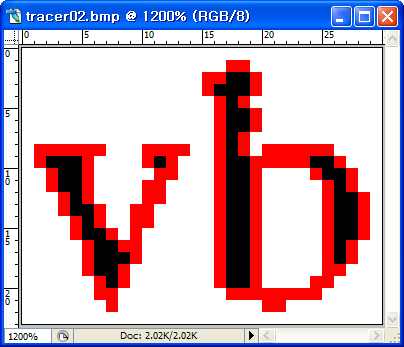
\includegraphics[width=0.3\textwidth]{5.ExperimentalResult/fig17-b.png} \label{fig:img17-b} }

	\caption{\JHMEMO{Visual comparison of two Contour Tracing Methods.} \protect\subref{fig:img17-a} MNT \protect\subref{fig:img17-b} Proposed method (without inner corners)}
	\label{fig:image17}
\end{figure}


%%%%%%%%%%%%%%%%%%%%%%%%%%%%%%%%%%%%%%%%%%%%%%%%%%%%%%%%%%%%%%%%%%%%%%%%%%%
\subsection{Speed}

% In order to measure the tracing time for each algorithm, we performed each algorithm 10 times per image and calculated the average time. We used the GetTickCount() function supported by Microsoft Visual C++ 6.0 to measure the processing time. Tables \textcolor{red}{8 and 9} show the average processing time of each algorithm used for tracing the images, and a linear model for estimating the process time as the number of traced pixels increases by using the least-square estimation (LSE) method. In the tables, the average processing time per traced contour pixel is obtained by dividing the total processing time by the total number of traced contour pixels. They are measured on the desktop and notebook separately.

In order to measure the tracing time for each algorithm, we performed each algorithm 10 times per image and calculated the average time. We used the \textit{cv2.getTickCount()} function supported by \textit{OpenCV 3.0.0} to measure the processing time. Tables \ref{table:table8} shows the average processing time of each algorithm used for tracing the images, and a linear model for estimating the process time as the number of traced pixels increases using the least-square estimation (LSE) method. In the tables, we obtain the average processing time per traced contour pixel by dividing the total processing time by the total number of traced contour pixels.

% Moreover, figure \textcolor{red}{18} illustrates a graph that uses data from tables \textcolor{red}{7 to 9}. As shown in figures \textcolor{red}{18 (a) and (b)}, the proposed algorithm had the best performance in the case of the desktop, i.e., it had the least average processing time and showed the least increase in the ratio of process time to number of traced contour pixels, as shown in the LSE. In particular, although the proposed algorithm traced most of the numerous contour pixels in each image, it has the best or good performance when compared with the conventional algorithms. On the contrary, the SBF had the least average processing time for images and the least ratio from the LSE in the case of the notebook, and the proposed algorithm is second in rank based on the average processing time and LSE. from these experimental results the SBF is not the best algorithm for the note book because the ratio of the number of traced contour pixels is only approximately $92\%$ of the proposed algorithm. Due to this reason, the proposed algorithm has better performance than the other algorithms for the number of traced contour pixels and the processing time.

% \JHMEMO{
Figure \ref{fig:image18} illustrates a graph that uses data from Tables \ref{table:table7}. As shown in Figures \ref{fig:image18}, the proposed algorithm has the best performance, i.e., it had the least average processing time and showed the smallest increase in the ratio of the process time to the number of traced contour pixels, as shown in the LSE. In particular, although the proposed algorithm traced most of the contour pixels in each image, it has the best or a good performance when compared to the conventional algorithms. Therefore, the proposed algorithm has a better performance than the other algorithms for the number of traced contour pixels and the processing time. 

% }

%%% Table 8
%!TEX root = ../Fast_Contour_Tracing_Algorithm.tex
% -*- root: ../Fast_Contour_Tracing_Algorithm.tex -*-

% Please add the following required packages to your document preamble:
% \usepackage{graphicx}

\definecolor{Gray}{gray}{0.85}

% \begin{table}[]
% \centering
% \caption{Speed Experimental Result (Unit: Seconds)}
% \label{table:table8}
% \resizebox{\textwidth}{!}{%
% % \begin{tabular}{p{0.14\textwidth}llllll}
% \begin{tabular}{p{0.14\textwidth}p{0.14\textwidth}p{0.14\textwidth}p{0.14\textwidth}p{0.14\textwidth}p{0.14\textwidth}p{0.14\textwidth}}
% \toprule

% Image                                 & Proposed Algorithm & ISBF        & MSBF        & SBF         & MNT         & RSA         \\
% \midrule
% \#1                                   & \cellcolor{Gray}0.00596            & 0.00622     & 0.00658     & 0.00626     & 0.00626     & 0.00750     \\
% \#2                                   & \cellcolor{Gray}0.00432            & 0.00562     & 0.00592     & 0.00468     & 0.00472     & 0.00560     \\
% \#3                                   & 0.00778            & 0.00808     & 0.00936     & \cellcolor{Gray}0.00752     & 0.00808     & 0.00940     \\
% \#4                                   & 0.01406            & 0.01500     & 0.01844     & \cellcolor{Gray}0.01346     & \cellcolor{Gray}0.01374     & 0.01842     \\
% \#5                                   & 0.00848            & 0.00908     & 0.01000     & 0.00866     & \cellcolor{Gray}0.00842     & 0.01000     \\
% \#6                                   & \cellcolor{Gray}0.00592            & 0.00684     & 0.00750     & 0.00658     & 0.00624     & 0.00686     \\
% \#7                                   & \cellcolor{Gray}0.01308            & 0.01470     & 0.01904     & 0.01376     & 0.01344     & 0.01748     \\
% \#8                                   & 0.00624            & 0.00688     & 0.00784     & \cellcolor{Gray}0.00622     & \cellcolor{Gray}0.00622     & 0.00656     \\
% \#9                                   & \cellcolor{Gray}0.01656            & 0.01874     & 0.02628     & 0.01778     & 0.01750     & 0.02188     \\
% \midrule
% Average                               & \cellcolor{Gray}0.00916            & 0.01013     & 0.01233     & 0.00944     & 0.00940     & 0.01152     \\
% \midrule
% Average time per traced contour pixel & \cellcolor{Gray}$4.91\times 10^{-8}$           & $5.43\times 10^{-8}$    & $7.19\times 10^{-8}$    & $5.50\times 10^{-8}$    & $6.18\times 10^{-8}$    & $7.57\times 10^{-8}$    \\
% \midrule
% LSE                                   & $3.23\times 10^{-8} + 0.0031$           & $3.57\times 10^{-8} + 0.0035$ & $5.74\times 10^{-8} + 0.0025$ & $3.58\times 10^{-8} + 0.0033$ & $4.06\times 10^{-8} + 0.0032$ & $5.54\times 10^{-8} + 0.0031$ \\
% R-square                              & 0.98117            & 0.98544     & 0.98838     & 0.98685     & 0.99461     & 0.97615    \\
% \bottomrule
% \multicolumn{7}{l}{\textsuperscript{*}\footnotesize{Results of best or faster than the proposed algorithm are marked as shadow.}}

% \end{tabular}
% }
% \end{table}

\begin{table}[]
\scriptsize
\centering
\caption{Speed Experimental Result (Unit: Seconds)}
\label{table:table8}
\resizebox{\textwidth}{!}{%
\begin{tabular}{p{0.14\textwidth}p{0.07\textwidth}p{0.07\textwidth}p{0.07\textwidth}p{0.07\textwidth}p{0.07\textwidth}p{0.07\textwidth}p{0.07\textwidth}p{0.07\textwidth}p{0.07\textwidth}p{0.07\textwidth}p{0.07\textwidth}p{0.07\textwidth}}
\toprule
\multirow{2}{*}{Image} & \multicolumn{2}{l}{Proposed Algorithm} & \multicolumn{2}{l}{ISBF} & \multicolumn{2}{l}{MSBF} & \multicolumn{2}{l}{SBF} & \multicolumn{2}{l}{MNT} & \multicolumn{2}{l}{RSA} \\
 & Mean & Std. Dev. & Mean & Std. Dev. & Mean & Std. Dev. & Mean & Std. Dev. & Mean & Std. Dev. & Mean & Std. Dev. \\
 \midrule
\#1 & \cellcolor{Gray}0.00596 & \cellcolor{Gray}0.00032 & 0.00622 & 0.00069 & 0.00658 & 0.00074 & 0.00626 & 0.00060 & 0.00626 & 0.00054 & 0.00750 & 0.00058 \\
\#2 & \cellcolor{Gray}0.00432 & 0.00040 & 0.00562 & 0.00047 & 0.00592 & \cellcolor{Gray}0.00005 & 0.00468 & 0.00044 & 0.00472 & \cellcolor{Gray}0.00026 & 0.00560 & \cellcolor{Gray}0.00034 \\
\#3 & 0.00778 & 0.00046 & 0.00808 & \cellcolor{Gray}0.00036 & 0.00936 & 0.00085 & \cellcolor{Gray}0.00752 & 0.00069 & 0.00808 & \cellcolor{Gray}0.00033 & 0.00940 & 0.00066 \\
\#4 & 0.01406 & \cellcolor{Gray}0.00006 & 0.01500 & 0.00099 & 0.01844 & 0.00100 & \cellcolor{Gray}0.01346 & \cellcolor{Gray}0.00006 & \cellcolor{Gray}0.01374 & 0.00075 & 0.01842 & 0.00074 \\
\#5 & 0.00848 & \cellcolor{Gray}0.00038 & 0.00908 & 0.00080 & 0.01000 & 0.00086 & 0.00866 & 0.00054 & \cellcolor{Gray}0.00842 & 0.00075 & 0.01000 & 0.00065 \\
\#6 & \cellcolor{Gray}0.00592 & \cellcolor{Gray}0.00056 & 0.00684 & 0.00074 & 0.00750 & 0.00070 & 0.00658 & 0.00062 & 0.00624 & 0.00072 & 0.00686 & 0.00058 \\
\#7 & \cellcolor{Gray}0.01308 & 0.00068 & 0.01470 & 0.00096 & 0.01904 & 0.00110 & 0.01376 & 0.00091 & 0.01344 & \cellcolor{Gray}0.00058 & 0.01748 & 0.00072 \\
\#8 & 0.00624 & 0.00067 & 0.00688 & \cellcolor{Gray}0.00062 & 0.00784 & \cellcolor{Gray}0.00065 & \cellcolor{Gray}0.00622 & 0.00068 & \cellcolor{Gray}0.00622 & 0.00068 & 0.00656 & \cellcolor{Gray}0.00061 \\
\#9 & \cellcolor{Gray}0.01656 & 0.00079 & 0.01874 & \cellcolor{Gray}0.00063 & 0.02628 & \cellcolor{Gray}0.00053 & 0.01778 & 0.00086 & 0.01750 & 0.00089 & 0.02188 & 0.00093 \\
\midrule
Average & \cellcolor{Gray}0.00916 &  & 0.01013 &  & 0.01233 &  & 0.00944 &  & 0.00940 &  & 0.01152 &  \\
\midrule
Average time per traced contour pixel & \cellcolor{Gray}$4.91\times 10^{-8}$ &  & $5.43\times 10^{-8}$ &  & $7.19\times 10^{-8}$ &  & $5.50\times 10^{-8}$ &  & $6.18\times 10^{-8}$ &  & $7.57\times 10^{-8}$ &  \\
\midrule
LSE & $3.23\times 10^{-8} + 0.0031$ &  & $3.57\times 10^{-8} + 0.0035$ &  & $5.74\times 10^{-8} + 0.0025$ &  & $3.58\times 10^{-8} + 0.0033$ &  & $4.06\times 10^{-8} + 0.0032$ &  & $5.54\times 10^{-8} + 0.0031$ &  \\
R-square & 0.98117 &  & 0.98544 &  & 0.98838 &  & 0.98685 &  & 0.99461 &  & 0.97615 &  \\
\bottomrule
\multicolumn{7}{l}{*Results of best or faster speed/smaller standard deviation than the proposed algorithm are marked as shadow.} &  &  &  &  &  & 
\end{tabular}
}
\end{table}

%%% Image 18
\begin{figure}[htbp]
	\centering
	\subfloat[]{ 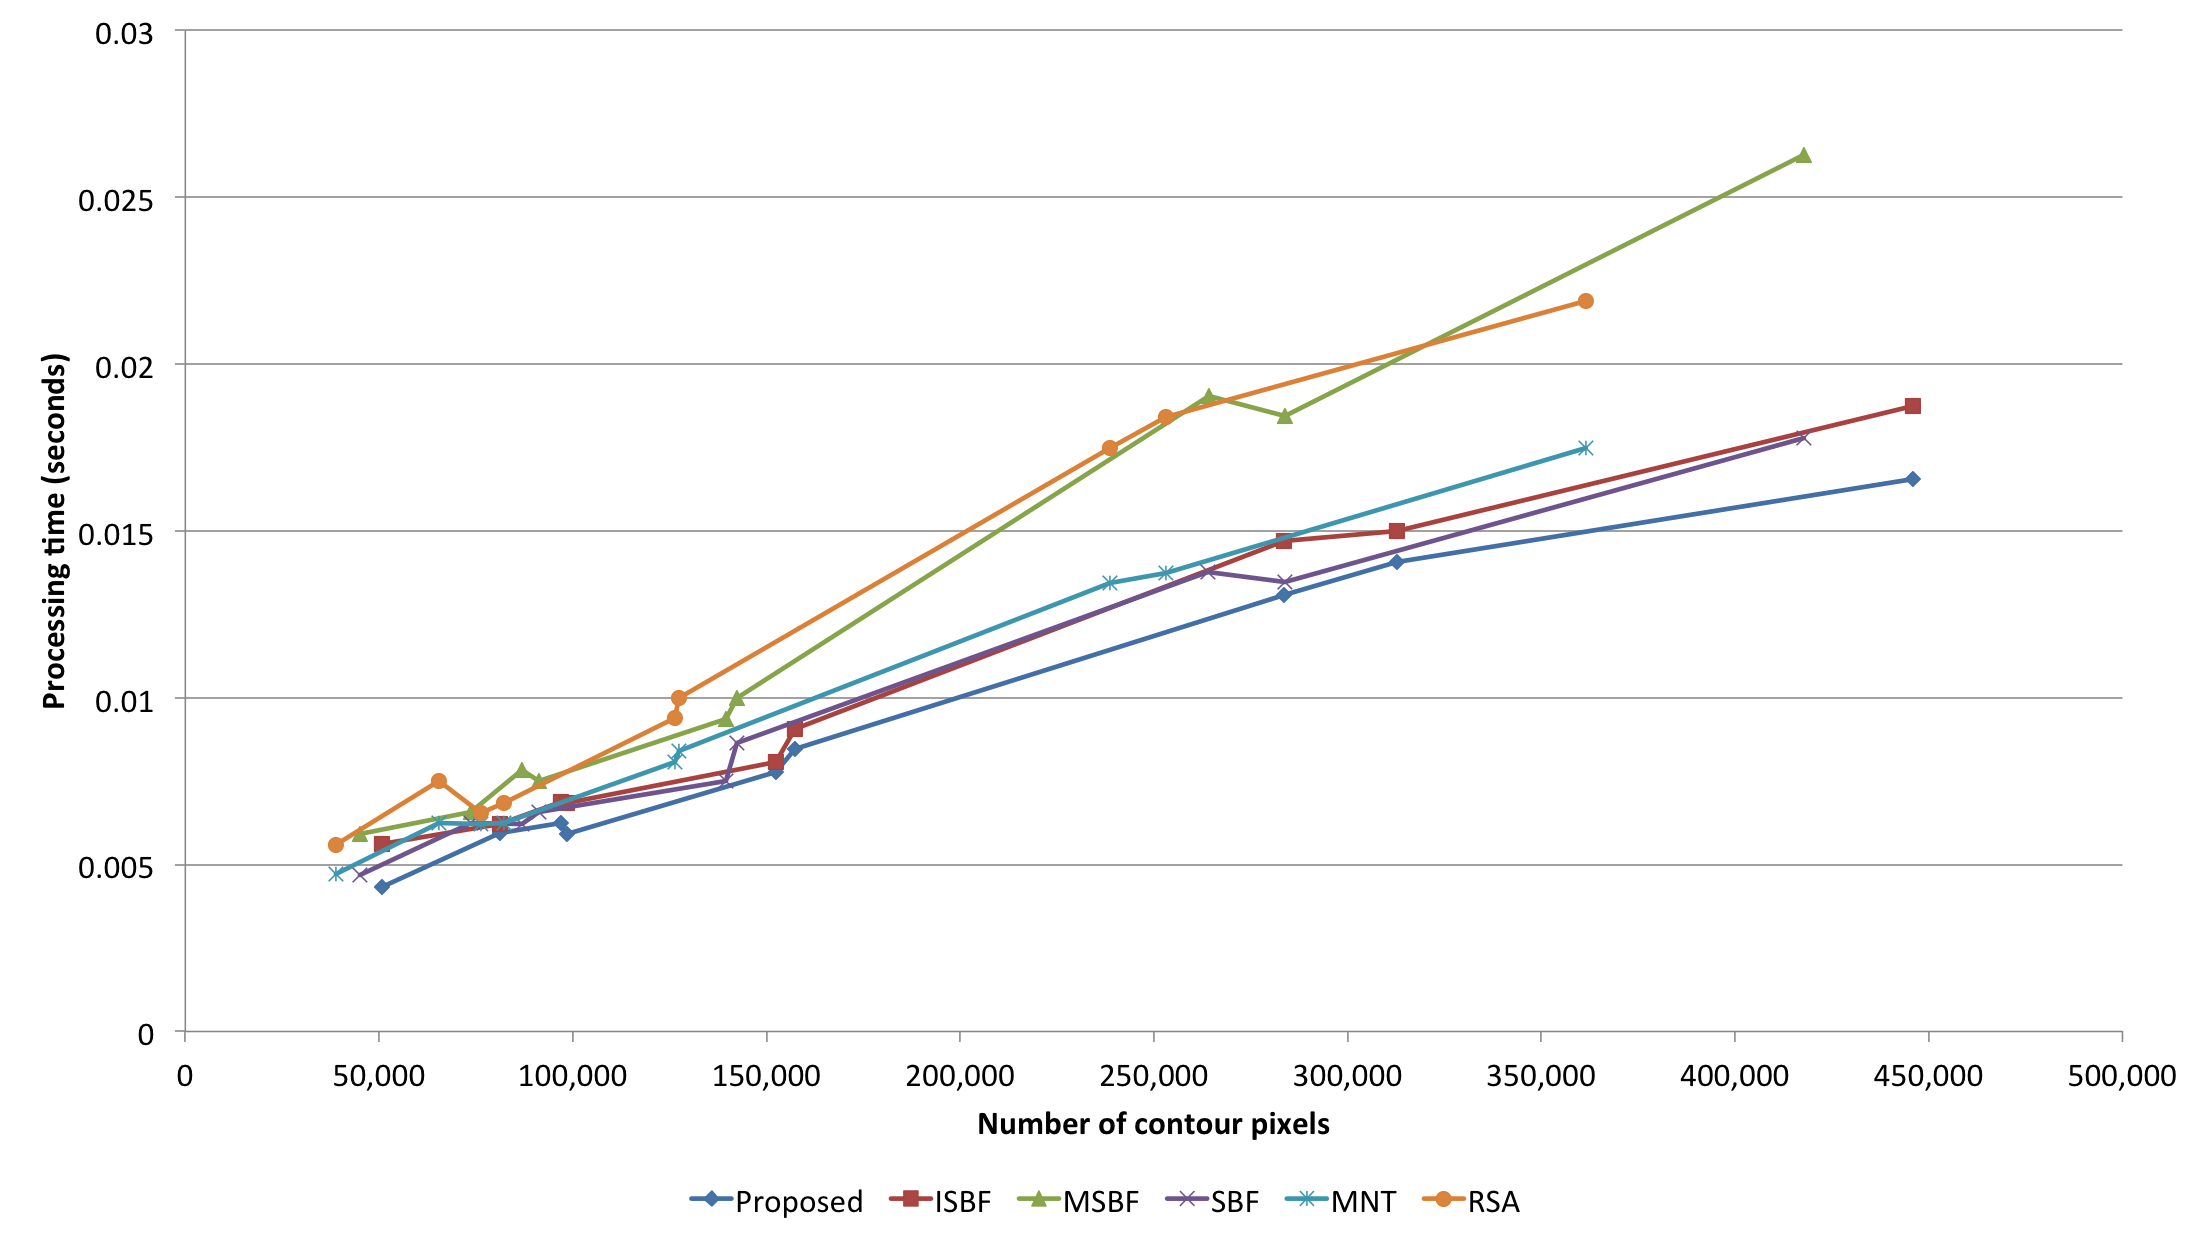
\includegraphics[width=.8\textwidth]{5.ExperimentalResult/fig18-a.png} \label{fig:img18-a} }\\
	\subfloat[]{ 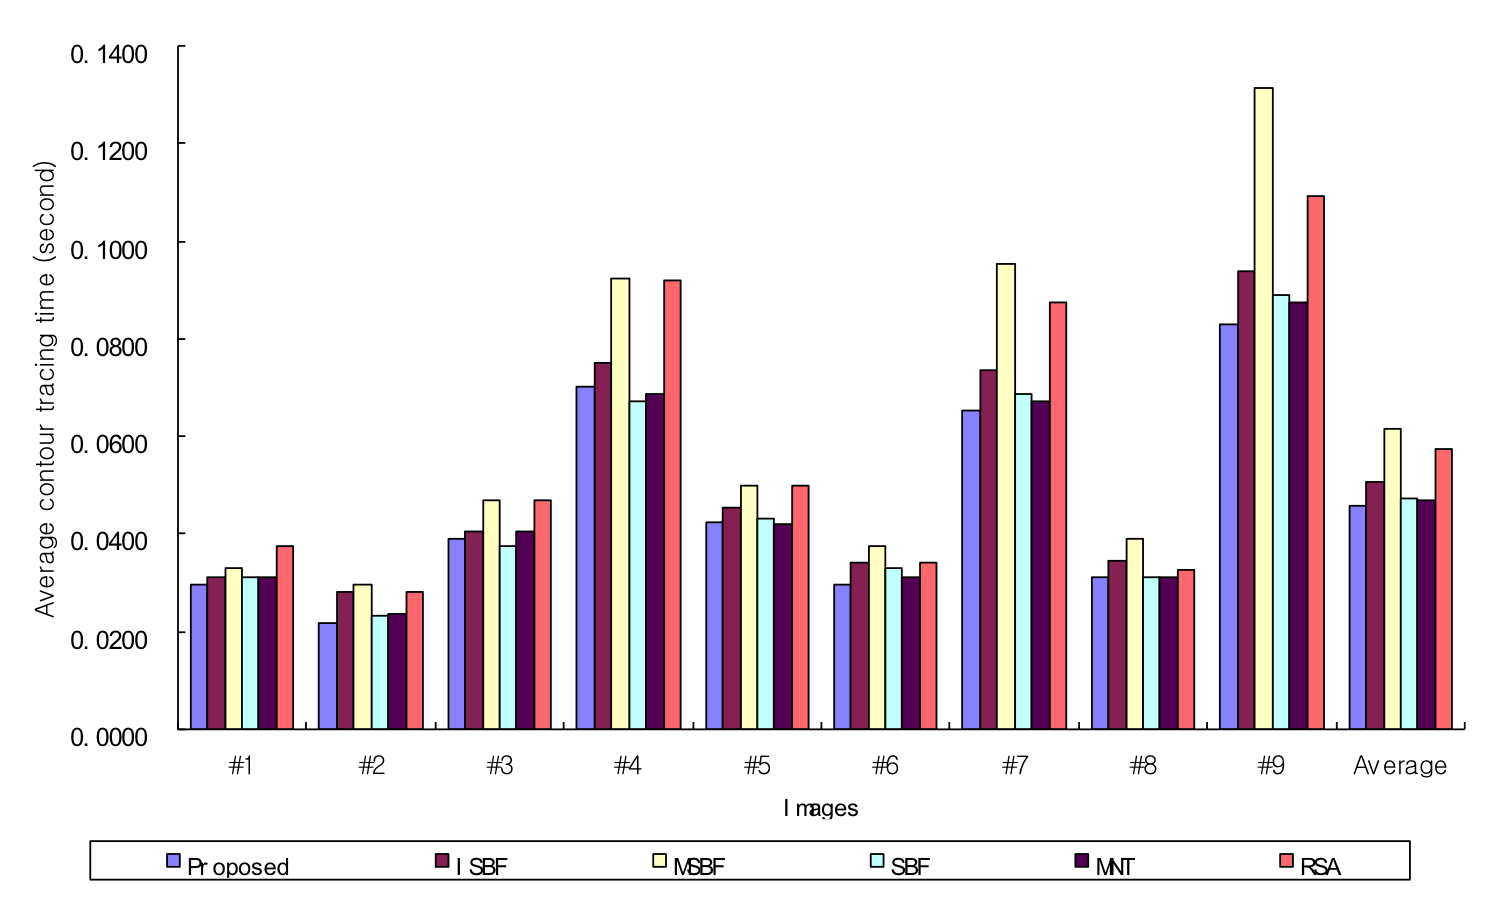
\includegraphics[width=.8\textwidth]{5.ExperimentalResult/fig18-b.png} \label{fig:img18-b} }

	\caption{Comparison of tracing times of contour tracing algorithms \protect\subref{fig:img18-a} Processing time vs. the number of contour pixels      \protect\subref{fig:img18-b} Average contour tracing time vs. images}
	\label{fig:image18}
\end{figure}



%%%%%%%%%%%%%%%%%%%%%%%%%%%%%%%%%%%%%%%%%%%%%%%%%%%%%%%%%%%%%%%%%%%%%%%%%%%
\subsection{Reduced Memory}

% The proposed algorithm does not save all the contour pixels, but it saves only the representative points and the inner-outer corner pixels. Table \textcolor{red}{10} shows the data size acquired from the above experiments on CCITT standard fax images. It shows the data sizes of traced contour pixels and its compressed data. The number of traced contour pixels $(A)$, which are same results from table \textcolor{red}{7} and the $C$ and $D$ in the table are numbers of the representative points and the inner-outer corner points of the traced contour pixels. $A$ and $C$ are the number of $(x, y)$ coordinates, and $D$ represents the number of inner-outer corners that comprise $(x, y)$ coordinates and the type of inner-outer corner. The benefit of storing only the representative points based on the vertex of the contour pixel is that it can dramatically reduce the data size. This experimental results showed that the proposed algorithm reduced the data size to {19~60\%} of the memory used when all the contour pixels were stored, as shown in Table \textcolor{red}{10}.

The proposed algorithm does not save all of the contour pixels, but it saves only the representative points and the inner-outer corner pixels. Table \ref{table:table10} shows the data size acquired from the above experiments performed using CCITT standard fax images. It shows the data sizes of traced contour pixels and their compressed data. The number of traced contour pixels (A), which are the same results from Table \ref{table:table7}, and $C$ and $D$ in the table indicate the number of representative points and inner-outer corner points of the traced contour pixels. $A$ and $C$ are the number of $(x, y)$ coordinates, and $D$ represents the number of inner-outer corners that comprise $(x, y)$ coordinates and the type of inner-outer corner. The benefit of storing only the representative points based on the vertex of the contour pixel is that it can significantly reduce the data size. The experimental results obtained show that the proposed algorithm reduced the data size to $19-60\%$ of the memory used when all of the contour pixels were stored, as shown in Table \ref{table:table10}.

%%% Table 10
%!TEX root = ../Fast_Contour_Tracing_Algorithm.tex
% -*- root: ../Fast_Contour_Tracing_Algorithm.tex -*-

% \begin{table}[]
% \scriptsize
% \centering
% \caption{Comparison Between Total Contour Pixels and Representative Points.}
% \label{table:table10}
% \begin{tabularx}{1.0\textwidth}{rR{2.1cm}R{2.0cm}R{2.9cm}R{3.0cm}R{2.5cm}R{2cm}}

% \toprule
% \multirow{2}{*}{} & \multicolumn{2}{l}{Entire contour pixels} & \multicolumn{3}{l}{Compressed data} & \multirow{2}{*}{Ratio ($\%$) ($E / B \times 100$) }	\\
% 				  & \multicolumn{1}{l}{Number of contour pixels ($A$)} & Data size ($B = A \times 2$) & Number of representative points ($C$) & Number of Inner outer corner points ($D$) & Data size ($E = C \times 2 + D \times 3$) & \\
% \midrule
% \#1               & 81,188                         & 162,376                      & 21,206                                & 61                                        & 42,595  & 26.23 \\
% \#2               & 50,824                         & 101,648                      & 12,695                                & 21                                        & 25,453  & 25.04 \\
% \#3               & 152,487                        & 304,974                      & 30,181                                & 53                                        & 60,521  & 19.84 \\
% \#4               & 312,812                        & 625,624                      & 86,953                                & 442    & 175,232 & 28.01 \\
% \#5               & 157,374                        & 314,748                      & 37,386                                & 113    & 75,111  & 23.86 \\
% \#6               & 98,566                         & 197,132                      & 18,464                                & 104    & 37,240  & 18.89 \\
% \#7               & 283,551                        & 567,102                      & 84,484                                & 1,539  & 173,585 & 30.61 \\
% \#8               & 97,015                         & 194,030                      & 21,928                                & 104    & 44,168  & 22.76 \\
% \#10              & 445,975                        & 891,950                      & 158,529                               & 75,425 & 543,333 & 60.92 \\
% \bottomrule

% \end{tabularx}
% \end{table}


% Please add the following required packages to your document preamble:
% \usepackage{multirow}
% \usepackage{graphicx}
\begin{table}[]
\centering
\caption{Comparison Between Total Contour Pixels and Representative Points.}
\label{table:table10}
\resizebox{\textwidth}{!}{%
\begin{tabular}{rrrrrrr}

\toprule

\multicolumn{1}{l}{} & \multicolumn{2}{l}{Entire contour pixels}                                                             & \multicolumn{3}{l}{Compressed data}                                   & \multicolumn{1}{l}{\multirow{2}{*}{\bigcell{Ratio ($\%$)\\($E / B \times 100$)}}} \\

\multicolumn{1}{l}{} & \bigcell{Number of\\contour pixels ($A$)} & \bigcell{Data size\\($B = A \times 2$)} & \bigcell{Number of\\representativepoints ($C$)} & \bigcell{Number of Inner outer\\corner points ($D$)} & \bigcell{Data size\\($E = C \times 2 + D \times 3$)} & \multicolumn{1}{l}{}                            \\


\midrule
\#1                  & 81,188                                             & 162,376                                          & 21,206                & 61                    & 42,595                & 26.23                                           \\
\#2                  & 50,824                                             & 101,648                                          & 12,695                & 21                    & 25,453                & 25.04                                           \\
\#3                  & 152,487                                            & 304,974                                          & 30,181                & 53                    & 60,521                & 19.84                                           \\
\#4                  & 312,812                                            & 625,624                                          & 86,953                & 442                   & 175,232               & 28.01                                           \\
\#5                  & 157,374                                            & 314,748                                          & 37,386                & 113                   & 75,111                & 23.86                                           \\
\#6                  & 98,566                                             & 197,132                                          & 18,464                & 104                   & 37,240                & 18.89                                           \\
\#7                  & 283,551                                            & 567,102                                          & 84,484                & 1,539                 & 173,585               & 30.61                                           \\
\#8                  & 97,015                                             & 194,030                                          & 21,928                & 104                   & 44,168                & 22.76                                           \\
\#10                 & 445,975                                            & 891,950                                          & 158,529               & 75,425                & 543,333               & 60.92                                          \\
\bottomrule
\end{tabular}
}
\end{table}

%%%%%%%%%%%%%%%%%%%%%%%%%%%%%%%%%%%%%%%%%%%%%%%%%%%%%%%%%%%%%%%%%%%%%%%%%%%
\subsection{Restoration}

% Figure \ref{fig:image19} shows an example of retrieval points and a restoration result obtained by using the proposed restoration algorithm. Figure \ref{fig:img19-a} is an example image that has all the contour pixel types, and it depicts the representative points and inner-outer corner points for contour description and restoration. This image has two contours, namely, an outer contour and an inner contour that includes two inner-outer corners. Table \textcolor{red}{11} describes these data and figure \textcolor{red}{18 (b)} shows the restoration results, which are retrieved using the data from table \textcolor{red}{11}. In the figure, the restored contour accurately represents the original contour pixels.

Figure \ref{fig:image19} shows an example of the retrieval points and a restoration result obtained using the proposed restoration algorithm. Figure \ref{fig:img19-a} is an example image that has all of the contour pixel types, and it depicts the representative points and inner-outer corner points for contour description and restoration. This image has two contours, namely an outer contour and an inner contour that includes two inner-outer corners. Table \ref{table:table11} describes these data and Figure \ref{fig:img19-b} shows the restoration results, which were retrieved using the data from Table \ref{table:table11}. In the figure, the restored contour accurately represents the original contour pixels.

%%% Image 19
\begin{figure}[htbp]
	\centering
	\subfloat[]{ 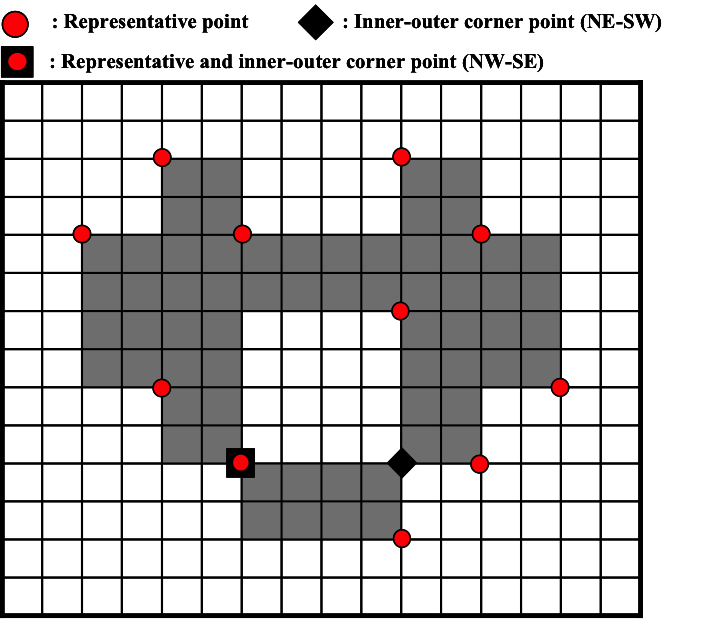
\includegraphics[width=7cm, height=6cm]{5.ExperimentalResult/fig19_a.png} \label{fig:img19-a} }
	\subfloat[]{ 
\includegraphics[width=7cm, height=5.25cm]{5.ExperimentalResult/fig19_b.png} \label{fig:img19-b} }
	 
	\caption{Example of Restoration of Contour Pixels. \protect\subref{fig:img19-a} Original image and its saved points for restoration      \protect\subref{fig:img19-b} Restoration by saved data}
	\label{fig:image19}
\end{figure}

%%% Table 11
%!TEX root = ../Fast_Contour_Tracing_Algorithm.tex
% -*- root: ../Fast_Contour_Tracing_Algorithm.tex -*-

% Please add the following required packages to your document preamble:
% \usepackage{multirow}
\begin{table}[]
\centering
\caption{Saved Data}
\label{table:table11}
\resizebox{\textwidth}{!}{%

\begin{tabular}{rrrllllllll}
\toprule
\multirow{3}{*}{i} & \multicolumn{5}{c}{Contour \#1. (outer contour)}                 & \multicolumn{5}{c}{Contour \#2. (inner contour)}                 \\ 
                   & \multicolumn{2}{c}{$R_i$} & \multicolumn{2}{c}{$C_i$} &          & \multicolumn{2}{c}{$R_i$} & \multicolumn{2}{c}{$C_i$} &          \\
                   & $x$           & $y$           & $x$           & $y$           & type     & $x$           & $y$           & $x$           & $y$           & type     \\
\midrule 
1                  & 3.5         & 1.5         & 9.5         & 9.5         & NE-SW    & 5.5         & 9.5         & 5.5         & 9.5         & NW-SE    \\
2                  & 5.5         & 3.5         & 5.5         & 9.5         & NW-SE    & 9.5         & 5.5         & 9.5         & 9.5         & NE-SW    \\
3                  & 9.5         & 1.5         &             &             &          &             &             &             &             &          \\
4                  & 11.5        & 3.5         &             &             &          &             &             &             &             &          \\
5                  & 13.5        & 7.5         &             &             &          &             &             &             &             &          \\
6                  & 11.5        & 9.5         &             &             &          &             &             &             &             &          \\
7                  & 9.5         & 11.5        &             &             &          &             &             &             &             &          \\
8                  & 5.5         & 9.5         &             &             &          &             &             &             &             &          \\
9                  & 3.5         & 7.5         &             &             &          &             &             &             &             &          \\
10                 & 1.5         & 3.5         &             &             &          &             &             &             &             &          \\
\bottomrule
\end{tabular}
}
\end{table}

% Figure \ref{fig:image20} shows the result for the CCITT \#1 image using the proposed restoration algorithm. Figure \ref{fig:img20-a} represents the result of contour tracing and \ref{fig:img20-b} depicts the result of restoration from the compressed contour data. To verify the identity, we compared the contour pixels of the two images and they are identical with regard to the number of contour pixels and the pixel coordinates, i.e., the contour pixels in the restoration result is the same as the original contour pixels. As shown in figures \ref{fig:image20} \textcolor{red}{figures 19 and 20}, these experiments proved that the proposed algorithm could trace the inner and outer contours, and it could store the results using lesser memory by storing only the representative points and inner-outer corner points instead of all the contour pixels; moreover, it could accurately restore all the contour pixels correctly from the compressed data. Besides, as shown in \cite{Miyatake1997Contour}, compressed data based on vertex contours guarantee precise enlarging.

Figure  \ref{fig:image20} shows the result obtained for the CCITT \#1 image using the proposed restoration algorithm. Figure \ref{fig:img20-a} represents the contour-tracing result, and \ref{fig:img20-b} depicts the result of restoration from the compressed contour data. To verify the identity, we compared the contour pixels of the two images, and found that they are identical with regard to the number of contour pixels and the pixel coordinates, i.e., the contour pixels in the restoration result are the same as the original contour pixels. As shown in Figures \ref{fig:image19} and \ref{fig:image20}, these experiments proved that the proposed algorithm could trace the inner and outer contours. Further, it was able to store the results using less memory by storing only the representative points and inner-outer corner points instead of all the contour pixels; moreover, it could correctly restore all the contour pixels from the compressed data. Besides, as shown in \cite{Miyatake1997Contour}, compressed data based on vertex contours guarantee precise enlarging.

%%% Image 20
\begin{figure}[htbp]
	\centering
	\subfloat[]{ 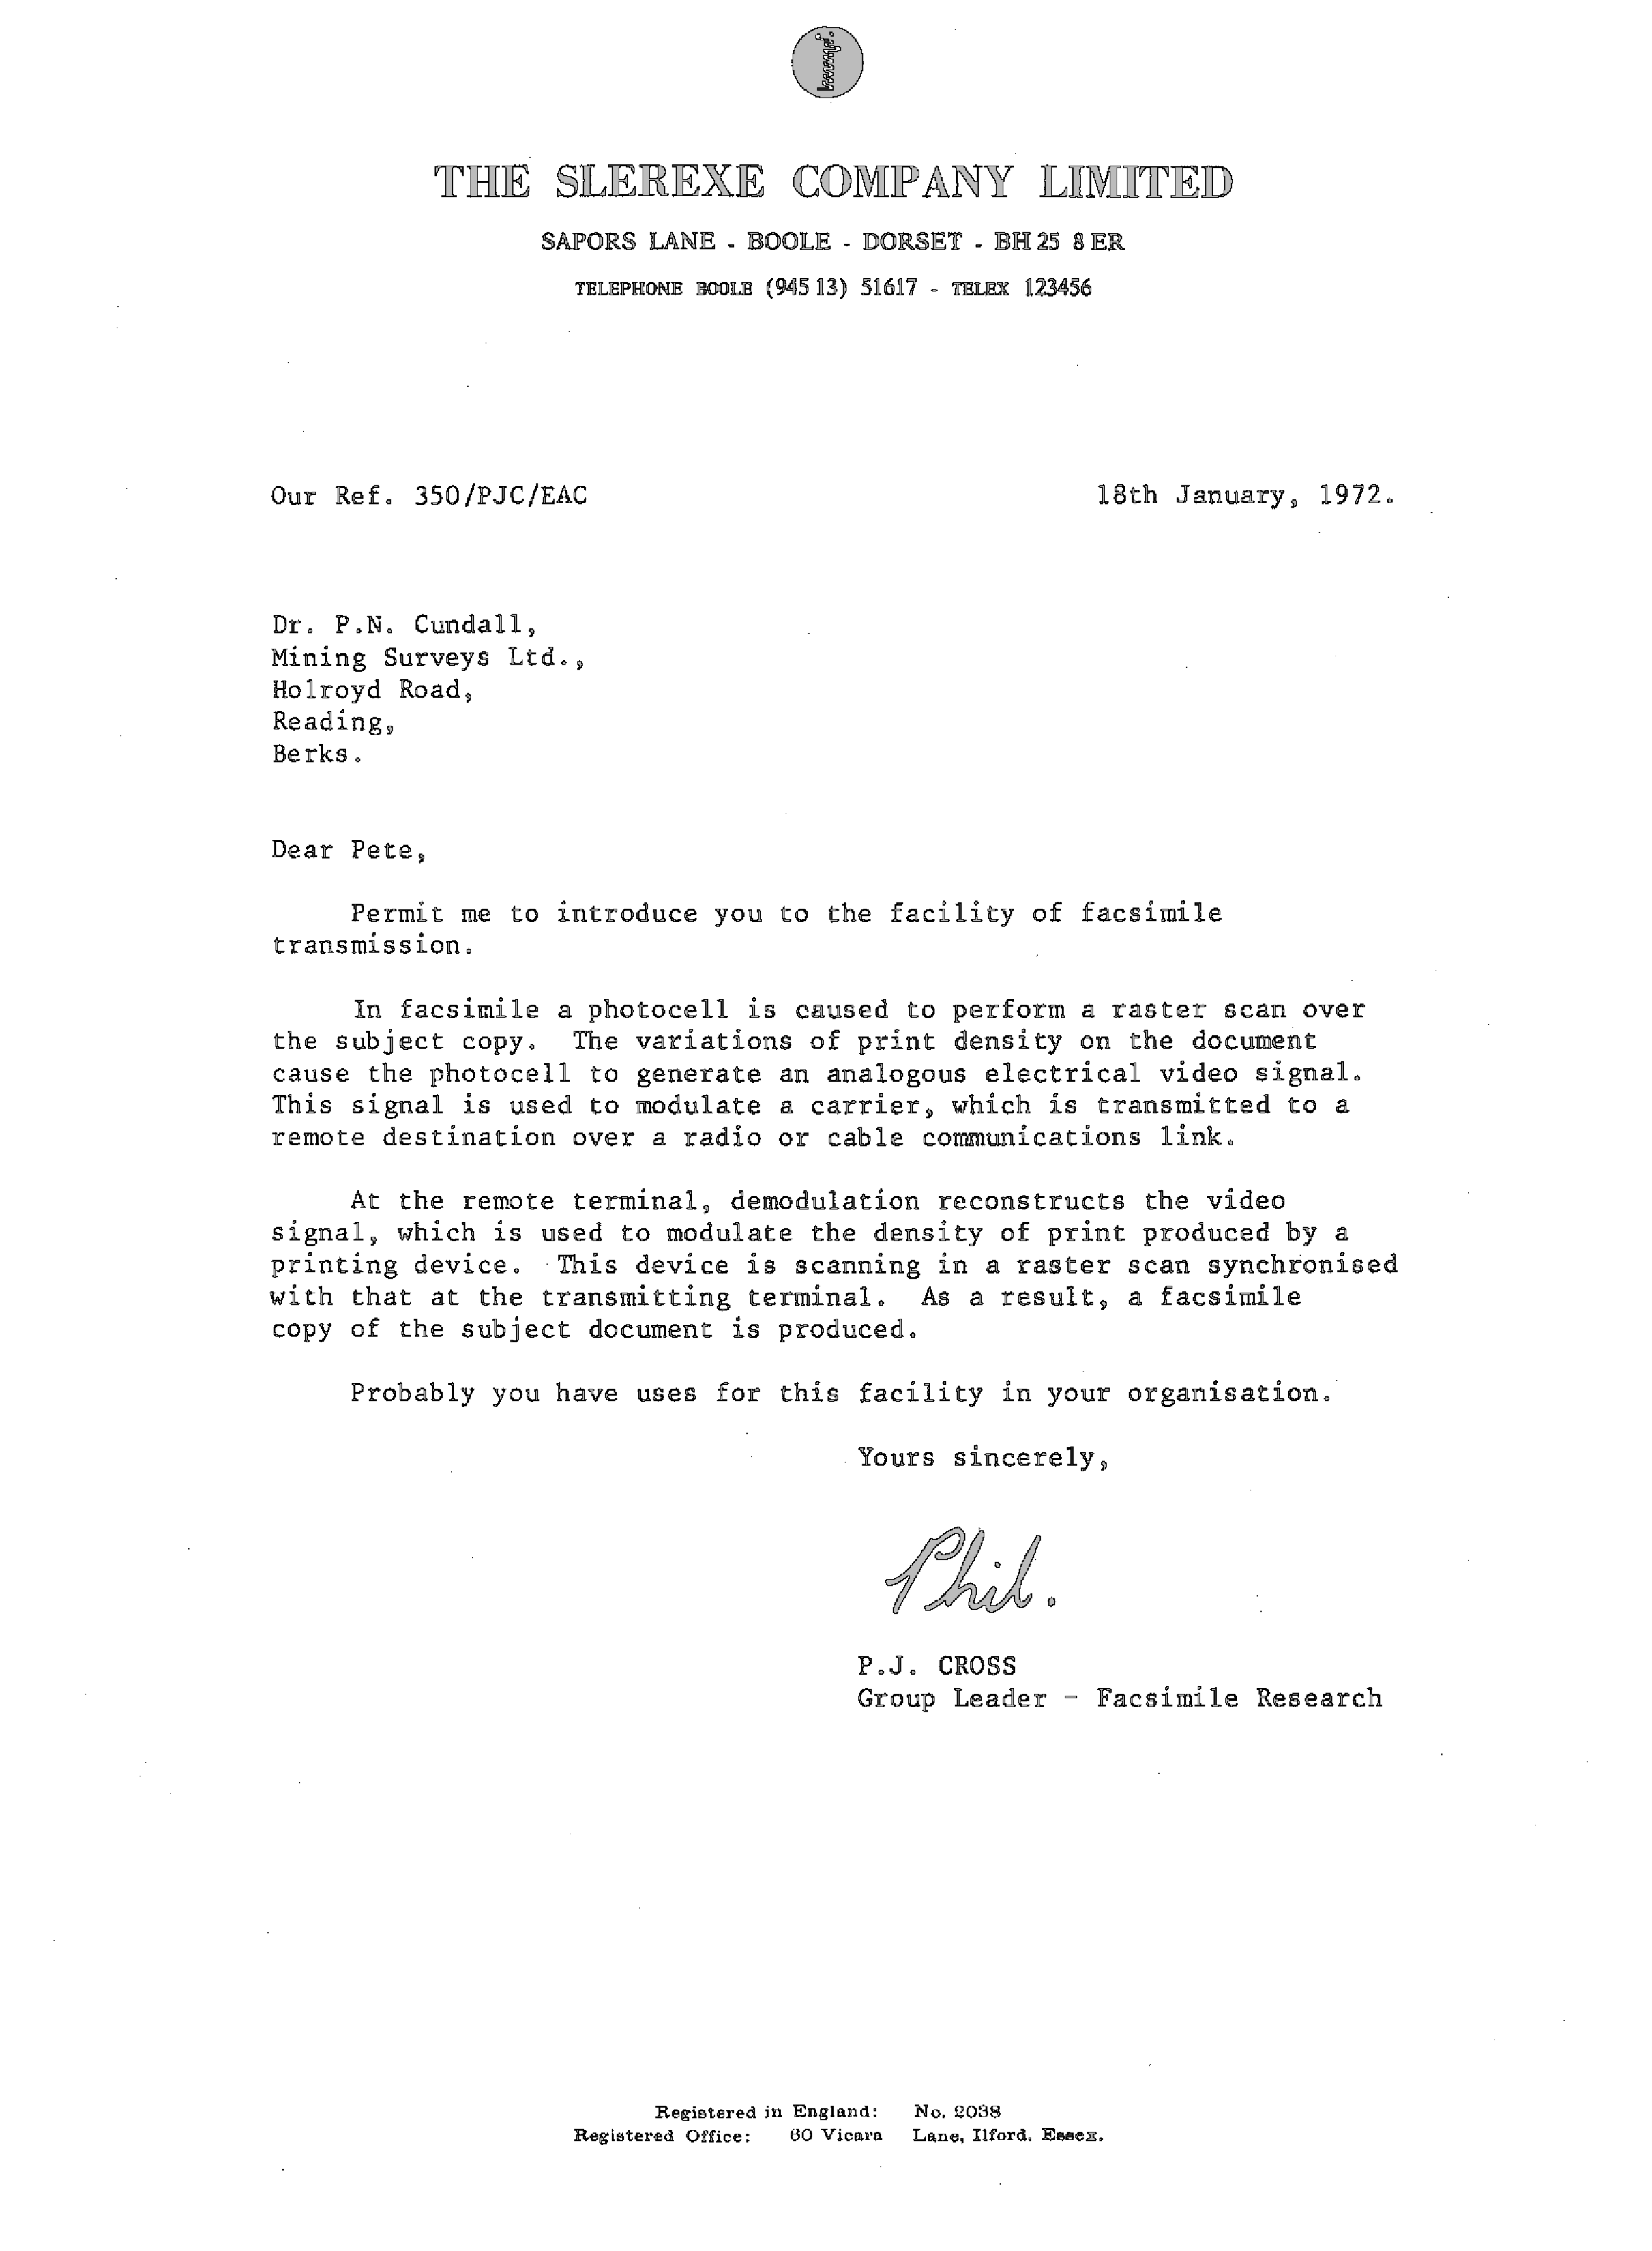
\includegraphics[width=0.5\textwidth]{5.ExperimentalResult/fig20_a.png} \label{fig:img20-a} }
	\subfloat[]{ 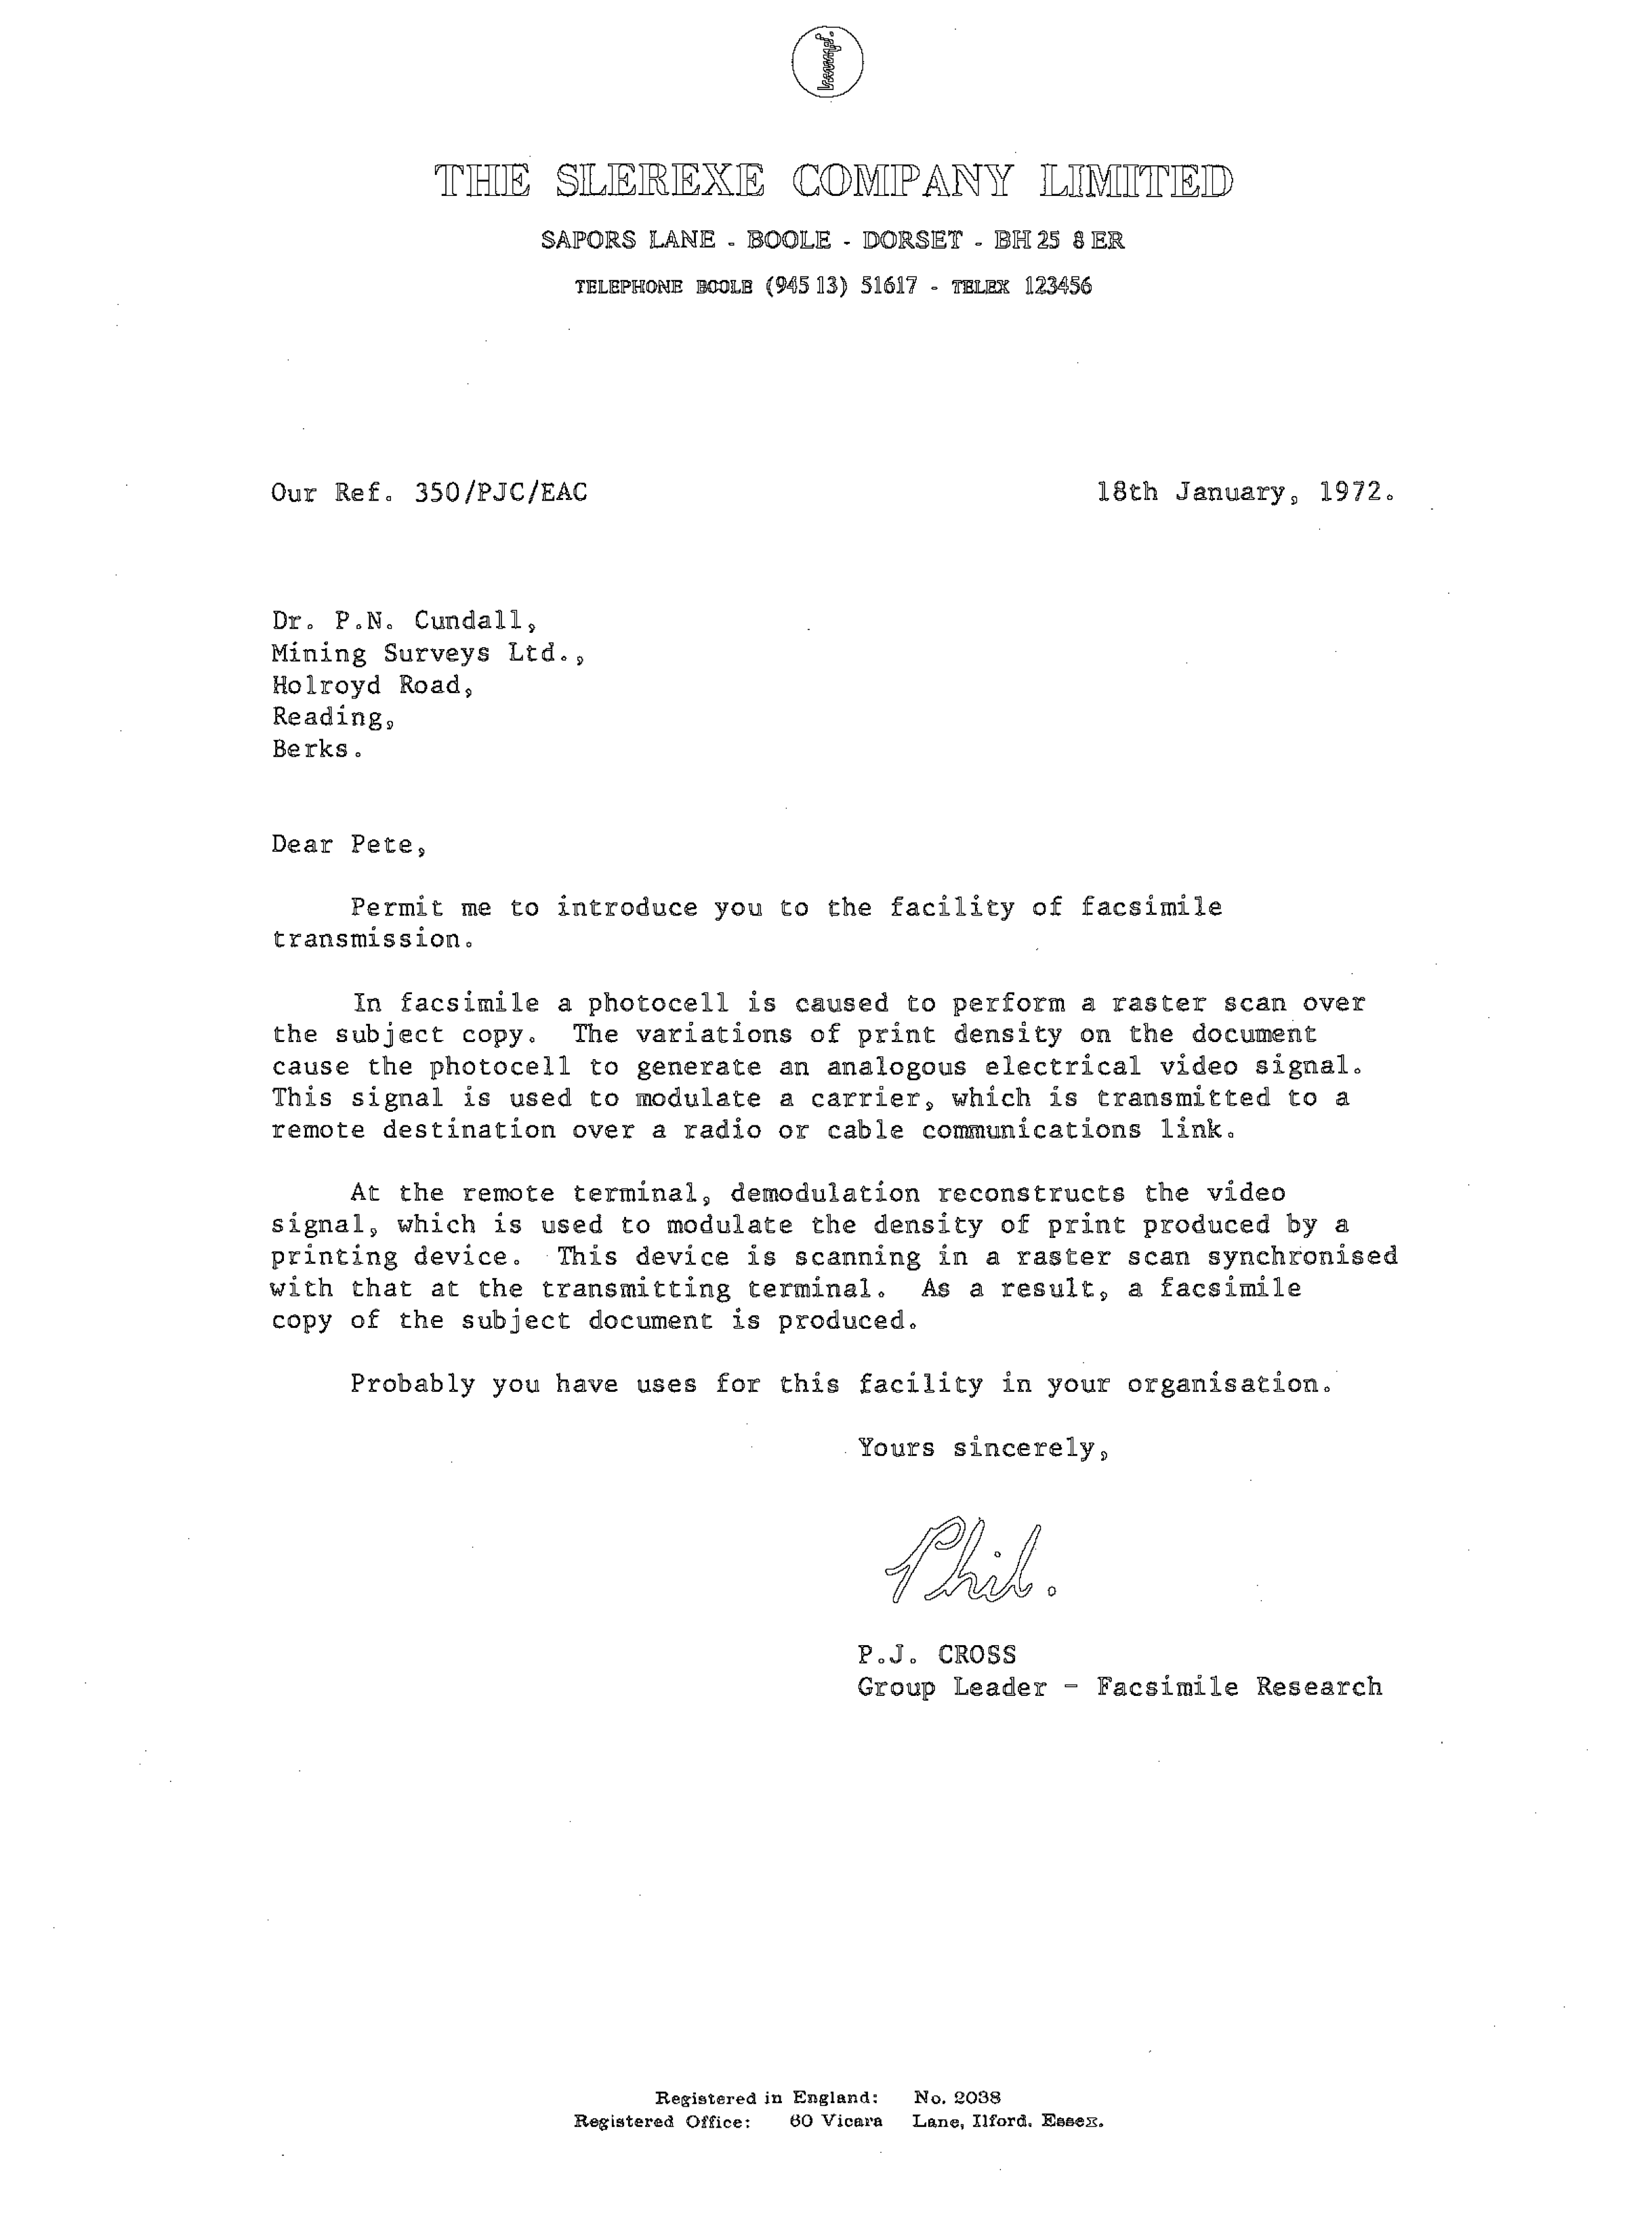
\includegraphics[width=0.5\textwidth]{5.ExperimentalResult/fig20_b.png} \label{fig:img20-b} }
	 
	\caption{Result of Experiment for CCITT \#1. Red Pixels are Contour Pixels. \protect\subref{fig:img20-a} Result of contour tracing \protect\subref{fig:img20-b} Result of contour restoration}
	\label{fig:image20}
\end{figure}



%%%%%%%%%%%%%%%%%%%%%%%%%%%%%%%%%%%%%%%%%%%%%%%%%%%%%%%%%%%%%%%%%
\subsection{Limitations}

%%% Image 21
\begin{figure}[htbp]
	\centering
	\subfloat[]{ 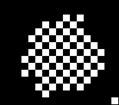
\includegraphics[width=4.5cm, height=4.5cm]{5.ExperimentalResult/fig21-a.png} \label{fig:img21-a} }
	\subfloat[]{ 
\includegraphics[width=4.5cm, height=4.5cm]{5.ExperimentalResult/fig21-b.png} \label{fig:img21-b} }
	\subfloat[]{ 
\includegraphics[width=4.5cm, height=4.5cm]{5.ExperimentalResult/fig21-c.png} \label{fig:img21-c} }
	 
	\caption{Example of Untraed Contour Pixels Caused by Missing Starting Pixel CCITT Image \#9 From $(1093, 1766)$ to $(1108, 1780)$. \protect\subref{fig:img21-a} Original image \protect\subref{fig:img21-b} Traced by ISBF \protect\subref{fig:img21-c} Traced by the proposed algorithm}
	\label{fig:image21}
\end{figure}

%%% Image 22
\begin{figure}[htbp]
	\centering
	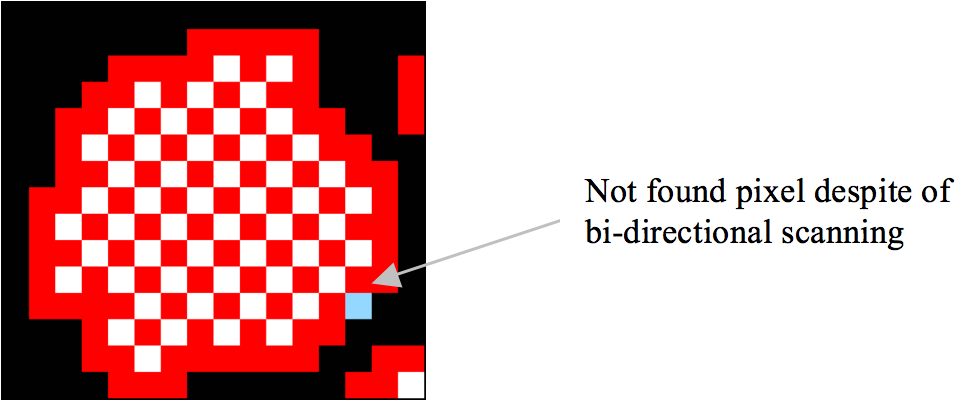
\includegraphics[width=0.6\textwidth]{5.ExperimentalResult/fig22.png}
	\caption{Result of Proposed Algorithm by using Bidirectional Scanning.}
	\label{fig:image22}
\end{figure}

% In the experiments, there were some missing contour pixels that did not satisfy the experimental conditions described in \cite{Danielsson1981Improvement}. In figures \ref{fig:img21-b} and \ref{fig:img21-c}, there are eight untraced contour pixels because the horizontal scan line cannot find a starting pixel for the contour under some conditions. In other words, since the scan line seeks an untraced black pixel with an adjacent white pixel on the horizontal line, if the untraced contour pixel which is between two black pixels in the horizontal direction has an adjacent white pixel in the vertical and/or diagonal direction, the untraced contour pixel cannot be considered as the starting pixel. Therefore, as shown in \textcolor{red}{Table 7}, the missing contour pixels remain after running the proposed algorithm and the untraced contour pixels of other algorithms are also included in the missing contour pixels due to the same problem. In particular, image \#9 has the largest number of missing contour pixels because it has many one-pixel-sized chessboard patterns that comprise inner-outer corner pixels. The chessboard pattern consists of one-pixel-sized inner-outer corner pixels, which tend to cause the missing start pixel problem. 

In the experiments, there were missing contour pixels that did not satisfy the experimental conditions described in \cite{Miyatake1997Contour}. In Figures \ref{fig:img21-b} and \ref{fig:img21-c}, there are eight untraced contour pixels because the horizontal scan line cannot find a starting pixel for the contour under certain conditions. In other words, because the scan line seeks an untraced black pixel with an adjacent white pixel on the horizontal line, if the untraced contour pixel that is between two black pixels in the horizontal direction has an adjacent white pixel in the vertical and/or diagonal direction, the untraced contour pixel cannot be considered as the starting pixel. Therefore, as shown in Table \ref{table:table7}, the missing contour pixels remain after running the proposed algorithm, and the untraced contour pixels of other algorithms are included in the missing contour pixels for the same reason. In particular, image \#9 has the largest number of missing contour pixels because it has many one-pixel-sized chessboard patterns that comprise inner-outer corner pixels. The chessboard pattern consists of one-pixel-sized inner-outer corner pixels, which tend to cause the missing start-pixel problem. 

% To overcome the problem, we can apply an 8 connection mask to the images for obtaining the starting pixel, but the mask requires many operations. In other words, we made an attempt to measure the performance of multidirection scanning for eliminating the missing contour pixels problem by using vertical and horizontal scans instead of 8 connection mask operation. \textcolor{red}{Table 12} shows the increase in the number of pixels traced by using bidirectional scanning, and \textcolor{red}{Table 13} describes the processing time for this method. Moreover, figure \ref{fig:image22} shows the tracing result obtained by using the proposed algorithm based on bidirectional scanning, and it shows that seven of the missing pixels are traced but still one diagonal connective contour pixel \textcolor{red}{(A)} is untraced. 


%%% Table 13

To overcome the problem, we applied an eight-connection mask to the images to obtain the starting pixel, but the mask required many operations. In other words, we attempted to measure the performance of multidirection scanning in order to eliminate the missing contour-pixel problem by using vertical and horizontal scans instead of an eight-connection mask operation. Table \ref{table:table12} shows the increase in the number of pixels traced using bidirectional scanning, and Table \ref{table:table13} describes the processing time for this method. Moreover, Figure \ref{fig:image22} shows the tracing result that was obtained using the proposed algorithm based on bidirectional scanning, and it shows that seven of the missing pixels are traced, but one diagonal connective-contour pixel (A) remained untraced. 

% In the above tables, bidirectional scanning slightly increases the number of traced contour pixels, but their processing time increases dramatically. Moreover, the proposed algorithm shows acceptable performance in terms of accuracy $(99.5\%)$, although only unidirectional scanning is performed. Hence, unidirectional scanning based on the proposed algorithm is sufficient for application to contour tracing under the condition that a relatively small number of objects are present and real-time tracing such as AR, MR, and recognition-image-based code is performed on small-scale images such as those in a mobile computing environment.

In the above tables, bidirectional scanning slightly increases the number of traced contour pixels, but their processing time increases significantly. Moreover, the proposed algorithm shows acceptable performance in terms of accuracy $(99.5\%)$, although we performed only unidirectional scanning. Hence, unidirectional scanning based on the proposed algorithm is sufficient for application to contour tracing under the condition that relatively few objects are present, and we performed real-time tracing such as AR, MR, and recognition-image-based code on small-scale images such as those in a mobile computing environment.

%!TEX root = ../Fast_Contour_Tracing_Algorithm.tex
% -*- root: ../Fast_Contour_Tracing_Algorithm.tex -*-

% Please add the following required packages to your document preamble:
% \usepackage{booktabs}
% \usepackage{multirow}
\begin{table}[]
\centering
\caption{Increases of Pixels Traced by Bidirectional Scan From One-directional Scan.}
\label{table:table12}

\resizebox{\textwidth}{!}{%

\begin{tabular}{@{}crrlrlrlrlrlrl@{}}
\toprule
      & \multirow{2}{*}{Total Number} & \multicolumn{2}{l}{Proposed} & \multicolumn{2}{l}{ISBF} & \multicolumn{2}{l}{MSBF} & \multicolumn{2}{l}{SBF} & \multicolumn{2}{l}{MNT} & \multicolumn{2}{l}{RSA} \\
      &                               & Number        & \%           & Number      & \%         & Number      & \%         & Number      & \%        & Number      & \%        & Number      & \%        \\ \midrule
\#1   & 81,189                        & 1             & 0.001        & 1           & 0.001      & 1           & 0.001      & 1           & 0.001     & 0           & 0.000     & 0           & 0.000     \\
\#2   & 50,825                        & 0             & 0.000        & 0           & 0.000      & 0           & 0.000      & 0           & 0.000     & 0           & 0.000     & 0           & 0.000     \\
\#3   & 152,489                       & 2             & 0.001        & 2           & 0.001      & 3           & 0.002      & 3           & 0.002     & 1           & 0.001     & 1           & 0.001     \\
\#4   & 312,812                       & 0             & 0.000        & 0           & 0.000      & 0           & 0.000      & 0           & 0.000     & 0           & 0.000     & 0           & 0.000     \\
\#5   & 157,377                       & 3             & 0.002        & 3           & 0.002      & 0           & 0.000      & 0           & 0.000     & 0           & 0.000     & 0           & 0.000     \\
\#6   & 98,579                        & 7             & 0.007        & 7           & 0.007      & 8           & 0.008      & 8           & 0.008     & 1           & 0.001     & 1           & 0.001     \\
\#7   & 283,717                       & 120           & 0.042        & 120         & 0.042      & 67          & 0.024      & 67          & 0.024     & 92          & 0.032     & 92          & 0.032     \\
\#8   & 97,031                        & 12            & 0.012        & 12          & 0.012      & 15          & 0.015      & 15          & 0.015     & 1           & 0.001     & 1           & 0.001     \\
\#9   & 453,721                       & 7,075         & 1.559        & 7,076       & 1.560      & 433         & 0.095      & 444         & 0.098     & 3,414       & 0.752     & 3,414       & 0.752     \\
Total & 1,687,740                     & 7,220         & 0.428        & 7,221       & 0.428      & 527         & 0.031      & 538         & 0.032     & 3,509       & 0.208     & 3,509       & 0.208     \\  
\bottomrule
\end{tabular}
}
\end{table}

%!TEX root = ../Fast_Contour_Tracing_Algorithm.tex
% -*- root: ../Fast_Contour_Tracing_Algorithm.tex -*-


% Please add the following required packages to your document preamble:
% \usepackage{multirow}
% \usepackage{graphicx}
\begin{table}[]
\centering
\caption{Computational Time Traced Bidirectionally}
\label{table:table13}

\resizebox{\textwidth}{!}{%
\begin{tabular}{lllllllllllll}
\toprule
\multirow{2}{*}{Image} & \multicolumn{2}{l}{Proposed} & ISBF            &       & MSBF            &       & SBF             &       & MNT             &       & RSA             &       \\
                       & Processing time    & Ratio   & Processing time & Ratio & Processing time & Ratio & Processing time & Ratio & Processing time & Ratio & Processing time & Ratio \\ \midrule
\#1                    & 0.064              & 2.1     & 0.067           & 2.2   & 0.074           & 2.2   & 0.064           & 2.0   & 0.067           & 2.1   & 0.069           & 1.8   \\
\#2                    & 0.061              & 2.8     & 0.063           & 2.2   & 0.061           & 2.1   & 0.056           & 2.4   & 0.061           & 2.6   & 0.067           & 2.4   \\
\#3                    & 0.072              & 1.9     & 0.083           & 2.1   & 0.084           & 1.8   & 0.077           & 2.0   & 0.077           & 1.9   & 0.083           & 1.8   \\
\#4                    & 0.11               & 1.6     & 0.116           & 1.5   & 0.131           & 1.4   & 0.109           & 1.6   & 0.111           & 1.6   & 0.135           & 1.5   \\
\#5                    & 0.078              & 1.8     & 0.084           & 1.9   & 0.089           & 1.8   & 0.078           & 1.8   & 0.078           & 1.9   & 0.089           & 1.8   \\
\#6                    & 0.065              & 2.2     & 0.073           & 2.1   & 0.075           & 2.0   & 0.064           & 1.9   & 0.07            & 2.2   & 0.072           & 2.1   \\
\#7                    & 0.108              & 1.7     & 0.111           & 1.5   & 0.134           & 1.4   & 0.11            & 1.6   & 0.113           & 1.7   & 0.125           & 1.4   \\
\#8                    & 0.069              & 2.2     & 0.07            & 2.0   & 0.074           & 1.9   & 0.067           & 2.2   & 0.067           & 2.2   & 0.075           & 2.3   \\
\#9                    & 0.128              & 1.5     & 0.139           & 1.5   & 0.172           & 1.3   & 0.127           & 1.4   & 0.13            & 1.5   & 0.147           & 1.3   \\
Total                  & 0.755              & 1.8     & 0.806           & 1.8   & 0.894           & 1.6   & 0.752           & 1.8   & 0.774           & 1.8   & 0.862           & 1.7   \\
\bottomrule

\end{tabular}
}
\end{table}

